\documentclass{beamer}
% foi retirada a opção -synctex=1
\usepackage[brazil]{babel}
\usepackage[T1]{fontenc}
\usepackage[utf8]{inputenc}
%\usepackage{graphicx}
%\usepackage{hyperref}
\usetheme{Madrid}
\usefonttheme[onlymath]{serif}
\usepackage{amssymb,amsfonts,amsmath,amsthm}
\usepackage{mathtools}
\usepackage{latexsym}
\usepackage[brazilian]{cleveref}

\usepackage{float}
\usepackage{indentfirst}
\usepackage{dsfont}
\usepackage{caption}
\usepackage{subcaption}

\DeclareMathOperator{\proj}{proj}
\DeclareMathOperator*{\argmax}{arg\, max}
\DeclareMathOperator*{\argmin}{arg\, min}
\DeclareMathOperator{\diag}{diag}
\DeclareMathOperator{\ones}{ones}

\def\Xset{\mathcal{X}}
\def\Yset{\mathcal{Y}}
\def\Hset{\mathcal{H}}
\def\RR{\mathds{R}}
\def\xbar{\bar{x}}
\def\wbar{\bar{w}}
\def\bbar{\bar{b}}


\newtheorem{teorema}{Teorema}%ambientes em itálico
\newtheorem{prop}{Proposição}
\newtheorem{teo}{Teorema}
\newtheorem{lema}{Lema}

\theoremstyle{definition}%ambientes normais
\newtheorem{exem}{Exemplo}[subsection]
\newtheorem{defi}{Definição}

\usepackage{csquotes}
\usepackage[
backend=biber,
style=numeric-comp, noerroretextools=true
]{biblatex}
\addbibresource{referencias.bib}

 \let\etoolboxforlistloop\forlistloop % save the good meaning of \forlistloop
 \usepackage{autonum}
 \let\forlistloop\etoolboxforlistloop % restore the good meaning of \forlistloop
 
 \title[Análise Teórica de SVM]{Análise Teórica de Máquinas de Vetores Suporte}
 \subtitle{Qualificação de TCC} 
 \author[Paula Ertel]{Aluna: Paula Cristina Rohr Ertel \\ Orientador: Luiz Rafael dos Santos}
 \institute[UFSC]{Universidade Federal de Santa Catarina - Campus Blumenau}
 \date{29 de Novembro de 2019}
 \logo{\includegraphics[width=0.1\textwidth]{UFSC.pdf}}
\begin{document}

\begin{frame}
	\maketitle
\end{frame}


\begin{frame}{Aprendizagem de Máquina}
\begin{itemize}
	%\item Motivação: Iniciar a apresentação comentando de como surgiu a ideia do tema para o TCC.
	\item A \textbf{Aprendizagem de Máquina} (do inglês \textit{Machine Learning}) é o estudo do uso de técnicas computacionais para automaticamente detectar padrões em dados e usá-los para fazer predições e tomar decisões.
	\begin{itemize}
		\item Aprendizagem Supervisionada.
		\item Aprendizagem não Supervisionada.	
	\end{itemize}
	\item Algumas aplicações da Aprendizagem de Máquina são:
	\begin{itemize} %site de referência https://www.sas.com/pt_br/insights/analytics/machine-learning.html
		\item Carros autônomos do Google.
		\item Recomendação de ofertas com base nas compras anteriores.
		\item Detecção de fraudes.
	\end{itemize}
\end{itemize}
\end{frame}


\begin{frame}{Máquinas de Vetores Suporte}
\begin{itemize}
	\item As \textbf{Máquinas de Vetores Suporte} (SVM, do inglês \textit{Support Vector Machine}) são uma técnica para aprendizagem supervisionada.

	\item Segundo \textcite{Evelin2017}, essa técnica foi desenvolvida por Vladimir Vapnik, Bernhard Boser, Isabelle Guyon e Corrina Cortes, com fundamentos provenientes da Teoria de Aprendizagem Estatística.
	
	\item Algumas aplicações de SVM em problemas práticos são o reconhecimento facial, leitura de placas automotivas e detecção de spam.
	%\item As SVM são indicadas nos casos em que ocorrem dados de dimensões elevadas e com altos níveis de ruídos, além de apresentar uma boa capacidade de generalização.

\end{itemize}
\end{frame}


\begin{frame}{Objetivo}
\begin{itemize}
	\item Estudar aspectos teóricos-matemáticos dos Métodos de Otimização relacionadas a Aprendizagem de Máquina \cite{Ana1994}, \cite{Solodov2014}, \cite{Izmailov2014}, \cite{Ademir2013}.

	\item Desenvolver um estudo teórico das Máquinas de Vetores Suporte \cite{Faisal2019}, \cite{Evelin2017}.

	\item Realizar uma implementação computacional da técnica de Máquinas de Vetores Suporte utilizando a linguagem de programação  \texttt{Julia}.
\end{itemize}
\end{frame}


\begin{frame}{SVM aplicada ao Problema de Classificação}

Considere um conjunto de dados, pertencentes a duas classes distintas, conforme \Cref{fig1}.

\begin{figure}[!h] 
	\centering
	\begin{subfigure}[h]{0.3\textwidth}
		\centering
		\includegraphics[width=\textwidth]{SVM_linear}
		\caption{Linear. \label{fig1:a}}
	\end{subfigure}
	\begin{subfigure}[!h]{0.3\textwidth}
		\centering
		\includegraphics[width=\textwidth]{SVM_flexivel}
		\caption{Flexível. \label{fig1:b}}
	\end{subfigure}
	\begin{subfigure}[!h]{0.3\textwidth}
		\centering
		\includegraphics[width=\textwidth]{SVM_naolinear}
		\caption{Não Linear. \label{fig1:c}}
	\end{subfigure}
	\caption{Dados lineares, com margem flexível e não lineares. \label{fig1}\\ Fonte: \textcite{Evelin2017}}
\end{figure}
\end{frame}


\begin{frame}{Uma Aplicação Prática}
\begin{figure}[H]
	\centering
	\begin{subfigure}[h]{0.8\textwidth}
		\centering
		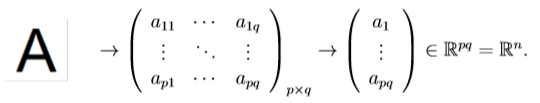
\includegraphics[width=\textwidth]{letraA_1.png}
	\end{subfigure}
	\begin{subfigure}[!h]{0.8\textwidth}
		\centering
		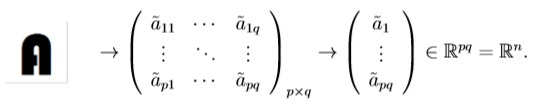
\includegraphics[width=\textwidth]{letraA_2.png}
	\end{subfigure}
	\begin{subfigure}[!h]{0.8\textwidth}
		\centering
		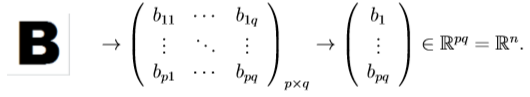
\includegraphics[width=\textwidth]{letraB.png}
	\end{subfigure}
	\caption{Classificação de caracteres. \\ Fonte: \textcite{Evelin2017}}
\end{figure}
\end{frame}


\begin{frame}
O problema de classificação trata-se de um problema de programação quadrática convexa com restrições lineares, que pode ser formulado como
\[
\begin{aligned}
\min_{w,b} & \quad f(w,b) \\
\text{s.a.} &  \quad g(w,b) \leq 0, \end{aligned}
\]
com $w\in \RR^n$ e $b\in \RR $, em que $f: \RR^n \rightarrow \RR$ é uma função quadrática e $g: \RR^{n+1} \rightarrow \RR^m$ é linear.

\end{frame}


\begin{frame}{Formulação Matemática do Problema de Classificação}
Considere os conjuntos de entrada $\Xset =\{x^1, \ldots , x^m \} \subset \RR^n$ e de treinamento $\Yset=\{(x^1, y_1), \ldots , (x^m, y_m)\mid x^i \in \Xset \, e \, y_i \in \{-1,1\}\}$, com a partição 
\[ \label{conj1}
\Xset ^{+} =\{x^i \in \Xset\mid y_i=1\} \quad e \quad \Xset^{-}=\{x^i \in \Xset\mid y_i=-1\},
\]
dos conjuntos formados pelos atributos pertencentes às classes positiva e negativa, respectivamente.

\begin{defi} Considere um vetor não nulo $w\in \RR^n$ e um escalar $b\in \RR$. Um hiperplano com vetor normal $w$ e constante $b$ é um conjunto da forma $\Hset(w,b)=\{x\in \RR^n \mid w^{T}x+b=0\}$.
\end{defi}
\end{frame}


\begin{frame}
\begin{figure}[h] 
	\centering
	\begin{subfigure}[h]{0.4\textwidth}
		\centering
		\includegraphics[width=\textwidth]{dados_treinamento}
		\caption{Dados de treinamento. \label{fig2:a}}
	\end{subfigure}
	\begin{subfigure}[h]{0.38\textwidth}
		\centering
		\includegraphics[width=\textwidth]{hiperplanos_separadores}
		\caption{Hiperplanos separadores. \label{fig2:b}}
	\end{subfigure}
	\caption{Conjunto de Dados e Hiperplanos. \label{fig2}
		\\ Fonte: \textcite{Evelin2017}}
\end{figure}
\end{frame}


\begin{frame}
\begin{figure}[h] 
	\centering
	\begin{subfigure}[h]{0.4\textwidth}
		\centering
		\includegraphics[width=\textwidth]{hiperplano_otimo}
		\caption{Hiperplano ótimo. \label{fig3:a}}
	\end{subfigure}
	\begin{subfigure}[h]{0.4\textwidth}
		\centering
		\includegraphics[width=\textwidth]{maxima_margem}
		\caption{Máxima margem. \label{fig3:b}}	
	\end{subfigure}
	\caption{Hiperplano Ótimo. \label{fig3}
		\\ Fonte: \textcite{Evelin2017}}
\end{figure}
\end{frame}


\begin{frame}{Conjuntos Linearmente Separáveis}
\begin{defi} \label{def1} Os conjuntos $\Xset^{+}, \Xset^{-} \subset \RR^n$ são ditos linearmente separáveis quando existem $w\in \RR^n$ e $b\in \RR$  tais que $w^{T}x+b>0$ para todo $x\in \Xset^{+}$ e $w^{T}x+b<0$ para todo $x\in \Xset^{-}$. O hiperplano $\Hset(w,b)$ é chamado hiperplano separador dos conjuntos $\Xset^{+}$ e $\Xset^{-}$.
\end{defi}
\end{frame}


\begin{frame}
\begin{lema} \label{lema1} Suponha que os conjuntos $\Xset^{+}, \Xset^{-} \subset \RR^n$ são finitos e linearmente separáveis, com hiperplano separador $\Hset(w,b)$. Então, existem $\overline{w}\in \RR^n$ e $\overline{b}\in \RR$ tais que $\Hset(w,b)$ pode ser descrito por
	\[
	\wbar^{T}x+\bbar =0,
	\]
	satisfazendo
	\begin{align}
	\wbar^{T}x+\bbar &\geq 1, \text{ para todo } x\in \Xset^{+}, \label{eq1} \\
	\wbar^{T}x+\bbar &\leq -1, \text{ para todo } x\in \Xset^{-}. \label{eq2}
	\end{align}
\end{lema} 
\end{frame}


\begin{frame}
Pelo \Cref{lema1} tem-se que $\Hset^{+}:=\{x\in \RR^n \mid w^{T}x+b= 1\}$ e $\Hset^{-}:=\{x\in \RR^n \mid w^{T}x+b= -1\}$ são os hiperplanos que definem a faixa que separa os conjuntos $\Xset^{+}$ e $\Xset^{-}$.

\begin{prop} \label{prop1} A projeção ortogonal de um vetor $\xbar\in \RR^n$ sobre um hiperplano afim $\Hset(w,b)$, é dada por
	\[ \proj_{\Hset}(\xbar)= \xbar - \dfrac{w^{T}\xbar+b}{w^{T}w}w. \]
	Além disso, a $\proj_{\Hset}(\xbar)$ satisfaz a menor distância.
\end{prop}
\end{frame}


\begin{frame}
O \Cref{lema2} estabelece a largura da faixa entre os hiperplanos separadores $\Hset^{+}$ e $\Hset^{-}$.

\begin{lema}\label{lema2} A distância entre os hiperplanos $\Hset^{+}$ e $\Hset^{-}$ é dada por $d=\dfrac{2}{\Vert w\Vert}.$
\end{lema}
\end{frame}


\begin{frame}
Para encontrar o hiperplano que melhor separa os dados é preciso maximizar $d=\dfrac{2}{\Vert w\Vert }$, ou equivalentemente, minimizar $\dfrac{1}{2}\Vert w\Vert^{2}$. 

Como a faixa deve separar os dados das duas classes, as seguintes restrições devem ser satisfeitas
\begin{align}
w^{T}x+b &\geq 1 , \text{ para  todo } x\in \Xset^{+}, \\
w^{T}x+b &\leq -1 , \text{ para  todo } x\in \Xset^{-}.
\end{align}

Reescrevendo as restrições acima de uma forma mais compacta temos
\[ y_{i}(w^{T}x^{i}+b)\geq 1, \quad i=1, \ldots ,m. \]
\end{frame}


\begin{frame}
Portanto, o problema de encontrar o hiperplano ótimo pode ser formulado da seguinte maneira
\[ \label{eq5}
\begin{aligned}
\min_{w,b} & \quad \dfrac{1}{2} \Vert w\Vert^{2} \\
\text{s.a.} &  \quad y_i(w^{T}x^{i}+b) \geq 1, \quad i=1, \ldots , m, \end{aligned}
\]
onde $w\in \RR^{n}$ e $b\in \RR$. 
\end{frame}


\begin{frame}{Projetos Futuros}
\begin{itemize}
	\item Estudar as condições de otimalidade para problemas com restrições.

	\item Estudar a teoria de dualidade, em particular a relacionada ao problema de programação quadrática.

	\item Realizar uma implementação computacional da técnica de Máquinas de Vetores Suporte a um problema de classificação utilizando a linguagem de programação \texttt{Julia}.
\end{itemize}
\end{frame}


\begin{frame}
\centering
\Large{Obrigada pela atenção!}
\end{frame}


\begin{frame}
\printbibliography
\end{frame}

\end{document}